\section{Evaluation}
%(partly) implementation of system or\\
%partly) Simulation of system e.g. in Matlab or microcontroller-based
%simulation of specific parts, or…

\subsection{Robot}
\label{Robot}
Die Klasse Robot stellt den Rescue Robot dar.\\
Zu Beginn verbindet sich der Robot in der \textbf{Methode makeSensors()} mit den acht Abstandsensoren, dem Wassersensor und dem Radiosensor. Dies ist auf Figur \ref{fig:makesensors} zu sehen. Dabei wird auch die dazugehörige Pinbelegung deklariert.\\
Für die Abstandssensoren wird eine Liste erstellt, zu der die acht Sensoren, inklusive Name,  Pinbelegung und Richtung, hinzugefügt werden.
\begin{figure}[htbp] 
  \centering
     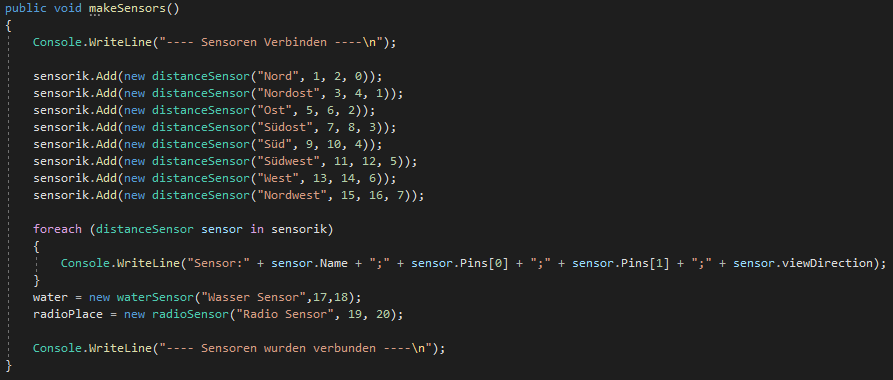
\includegraphics[width=0.5\textwidth]{Bilder/makeSensors.PNG}
  \caption{Methode makeSensors()}
  \label{fig:makesensors}
\end{figure}\\
Figur \ref{fig:drive} zeigt die \textbf{Methode drive()}. In der Methode drive() wird ein Zufallswert zwischen 0 und 2 generiert, welcher dann in einer If-else-Anweisung über den zu fahrenden Weg des Rescue Robots entscheidet. Ist der zufällig generierte Wert null, so fährt der Rescue Robot den kurzen Weg, sonst fährt er den lange Weg.\\
In jedem Fall greift die Methode drive() auf die Liste der eingelesenen Referenzpunkte zurück, welche der Rescue Robot abfährt.
\begin{figure}[htbp] 
  \centering
     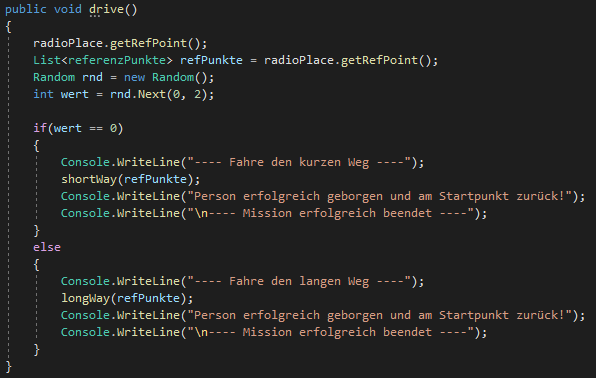
\includegraphics[width=0.4\textwidth]{Bilder/drive.PNG}
  \caption{Methode drive()}
  \label{fig:drive}
\end{figure}\\
Die \textbf{Methode fahreVonBis()}, zu sehen auf Figur \ref{fig:fahrevonbis}, greift auf die Methode getWay() in der Datei RobotLogic (siehe \ref{robotlogic}) zu, um den zu fahrenden Weg von einem Signalposten zum Anderen mit Rücksicht auf die Hindernisse zu berechnen. Diese Methode fahreVonBis() führt mithilfe eines Additionszuweisungsoperator (siehe Figur \ref{fig:fahrevonbis} gesamtWeg += p4.distance;) dazu, dass der gesamte Weg abgefahren wird. Zudem wird auch übergeben, was der zu befahrende Untergrund ist (siehe Figur \ref{fig:fahrevonbis} power.drive(startpos[0], startpos[1], p4.direction, p4.distance, water);).
\begin{figure}[htbp] 
  \centering
     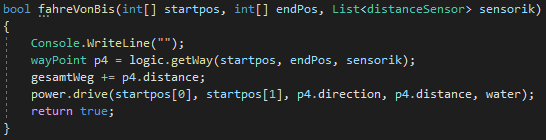
\includegraphics[width=0.4\textwidth]{Bilder/fahreVonBis.PNG}
  \caption{Methode fahreVonBis()}
  \label{fig:fahrevonbis}
\end{figure}\\
Der zu fahrende Weg wird in zwei zusätzlichen Methoden definiert, da es zwei mögliche Wege gibt. Der kurze Weg ist in der \textbf{Methode shortWay()} deklariert und der lange Weg ist in der \textbf{Methode longWay()} deklariert. Der Aufbau der beiden Methoden ist vom Prinzip gleich, in der Methode longWay() werden nur mehrere Sinalposten abgefahren als in der Methode shortWay().\\
Die genannten Methoden greifen auf die vorherige erläuterte Methode fahreVonBis() zu. Figur \ref{fig:shortway} zeigt die Methode shortWay(). Der Robot fährt zuerst von dem dritten Referenzpunkt, welcher dem Startpunkt entspricht, zum zweiten Referenzpunkt, welcher der zu bergenden Person entspricht. Daraufhin wird die Person identifiziert und die Livesteuerung wird aktiviert. Nachdem die Person erfolgreich per Livesteuerung des Roboterarms in dem Rescue Robot ist, fährt der Robot zurück von dem zweiten Referenzpunkt (geborgene Person) zum dritten Referenzpunkt (Startpunkt). Da die Referenzpunkte aus einem X- und einem Y-Wert bestehen, sind sie als Arrays definiert. Zum Schluss gibt die Methode noch den in der Methode fahreVonBis() errechneten zurückgelegten Gesamtweg aus.
\begin{figure}[htbp] 
  \centering
     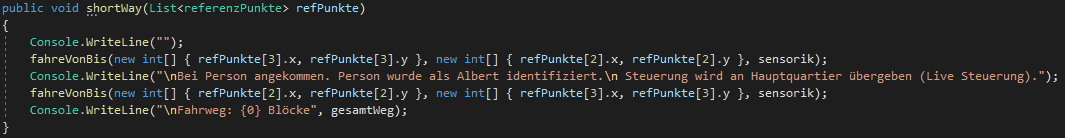
\includegraphics[width=0.5\textwidth]{Bilder/shortWay.PNG}
  \caption{Methode shortWay()}
  \label{fig:shortway}
\end{figure}
\begin{flushright}
	$ [ $Katrin Glöwing$ ] $
\end{flushright}


\subsection{Robot Logik}
\label{robotlogic}

Die Datei robotLogic besteht aus einer \textbf{Klasse wayPoint} und einer \textbf{Klasse Logic}.\\
Die \textbf{Klasse wayPoint} (siehe Figur \ref{fig:waypoint}) definiert eine Methode wayPoint() mit den Variablen der Richtung und der Distanz. Zudem werden die Variablen für die Erreichbarkeit des nächsten Signals und der Hindernisse deklariert.
\begin{figure}[htbp] 
  \centering
     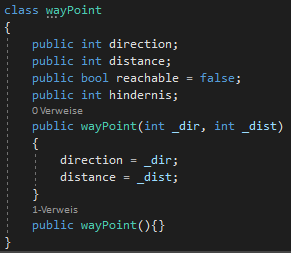
\includegraphics[width=0.2\textwidth]{Bilder/wayPoint.PNG}
  \caption{Methode wayPoint()}
  \label{fig:waypoint}
\end{figure}\\
Die eigentliche Logik des Robots ist in der \textbf{Klasse Logic} definiert. \\
Figur \ref{fig:fahren} zeigt die \textbf{Methode fahren()}, welche das Array move mit dem Inhalt der Richtung und der Distanz, die der Robot fahren soll, enthält.
\begin{figure}[htbp] 
  \centering
     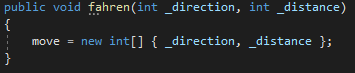
\includegraphics[width=0.3\textwidth]{Bilder/fahren.PNG}
  \caption{Methode fahren()}
  \label{fig:fahren}
\end{figure}\\
In der \textbf{Methode calcDirDist()} (siehe Figur \ref{fig:calcdirdist}) wird die Richtung, in die der Rescue Robot fahren soll und die Distanz, die der Robot zurücklegen soll, jeweils für die X- und Y-Koordinaten, ermittelt.\\
Die Variablen deltaX und deltaY entsprechen den Werten der zu fahrenden Distanz in X- und Y-Richtung. Mit einer If-elseif-Anweisung wird jeweils für den X- und den Y-Wert festgelegt, in welche Richtung der Robot welche Distanz zurücklegen soll. Mit den Zuweisungen point.direction=direction und point.distance=distance wird festgelegt, dass die If-elseif-Anweisungen immer für die aktuelle Position ausgeführt wird. Dafür wird point als aktuelle Position aus der Methode wayPoint (siehe Figur \ref{fig:waypoint}) verwendet.
\begin{figure}[htbp] 
  \centering
     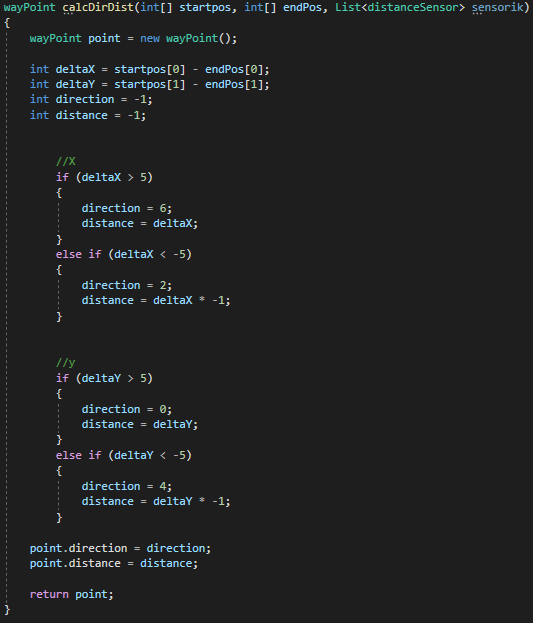
\includegraphics[width=0.3\textwidth]{Bilder/calcDirDist.PNG}
  \caption{Methode calcDirDist()}
  \label{fig:calcdirdist}
\end{figure}\\
Figur \ref{fig:getway} zeigt die \textbf{Methode getWay()}, welche den Abstand zum nächstliegenden Objekt, sei es eine Wand oder ein Hindernis, ermittelt.\\
Diese Methode greift auf die Informationen der Methode clacDirDist() zu, um die Richtung und die Entfernung (Werte entsprechen der Luftlinie), in die der Abstand zum nächstliegenden Objekt berechnet werden soll, zu erfahren. Daraufhin wird der Distanzsensor aus der Datei Sensoren (beschrieben von Domenic Drechsel) abgefragt, wie weit die Distanz zum nächsten Objekt (Wand oder Hindernis) ist. Mit einer If-else-Anweisung wird ermittelt ob die Entfernung aus der Methode calcDirDist() größer ist als die Strecke bis zum nächsten Objekt. Ist dies der Fall, so ist der von der Methode calcDirDist() ermittelte Zielpunkt nicht erreichbar und es ist ein Hindernis im Weg. Ist dies nicht der Fall, ist kein Hindernis im Weg und der Zielpunkt ist erreichbar.
\begin{figure}[htbp] 
  \centering
     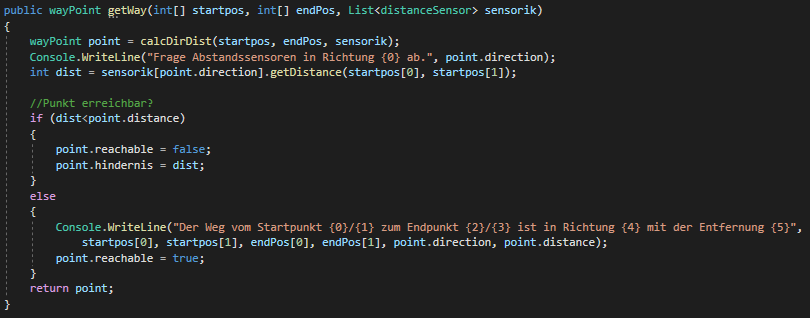
\includegraphics[width=0.5\textwidth]{Bilder/getWay.PNG}
  \caption{Methode getWay()}
  \label{fig:getway}
\end{figure}
\begin{flushright}
	$ [ $Katrin Glöwing$ ] $
\end{flushright}